
%%%%%%%%%%%%%%%%%%%%%%%%%%%%%%%%%%%%%%%%%%%%%%%%%%%%%%%%%%%%%
\begin{frame} [plain]
    \frametitle{}
    \Background[1] 
    \begin{center}
    {\huge 第6-7讲:相干态}
    \end{center}  
    \addtocounter{framenumber}{-1}   
\end{frame}
%%%%%%%%%%%%%%%%%%%%%%%%%%%%%%%%%%%%%%%%%%%%%%%%%%%%%%%%%%%% 

\section{1. 相干态的定义}

\begin{frame}
 \frametitle{相干态的定义}
 相干态: 也叫做格劳伯态, 是罗伊·格劳伯于1963年提出来的一种量子力学纯态, 它是数态的相干叠加态. (2005年诺贝尔物理学奖)。
 \[ \rs{\alpha} = \sum_{n=0} ^{+\infty} c_n  \rs{n} = e^{-\frac{1}{2}\left|\alpha\right|^2}  \sum_{n=0} ^{+\infty}  \frac{\alpha^n}{\sqrt{n!}} \rs{n} \]
   \begin{center}
        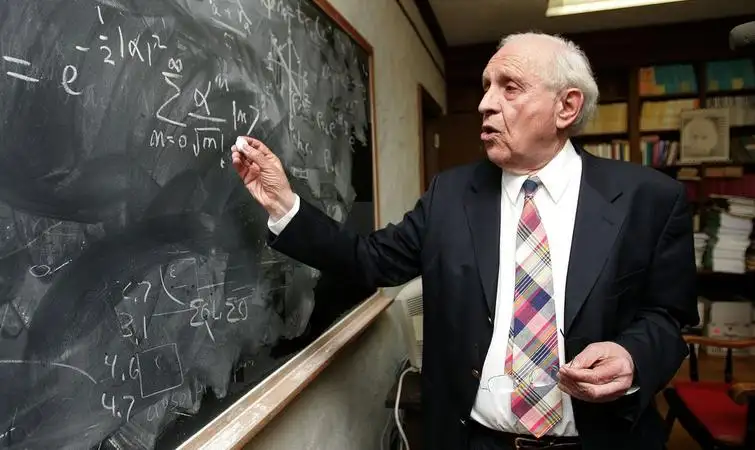
\includegraphics[width=0.5\textwidth]{figs/2022-04-27-11-50-32.png}
   \end{center}
\end{frame}

%\begin{frame}
% \frametitle{相干的经典经验}
%    经典相干三条件: 频率相同, 相差恒定, 传播方向相同.
% \begin{itemize}
%     \item 电谐振动的振动模式的空间传播形成电磁波
%     \item 频率相同的波是相干波
%     \item 谐振子拉离平衡位置(平移), 然后舒放 (起振)
%     \item 起振后谐振子的频率与拉离的距离无关 (固有频率)
%     \item 谐振子的能量与拉离的距离有关
% \end{itemize}
%    经验: 平移(拉离平衡位置) 产生相干态!    
%\end{frame}


\begin{frame} 
    \begin{tcolorbox4}[相干态基本命题:]
        \begin{enumerate}
            \item 湮灭算符的本征态是光场相干态
            \[ \hat{a}\rs{\alpha}= \alpha\rs{\alpha}\]
            \item 光场相干态源于真空态的平移
            \[ \hat{a} =  D(\alpha)  \rs{0}  \]
            \item 光场相干态具有超完备性
            \[ \frac{1}{\pi} \int \rl{\alpha}{\alpha}d ^2 \alpha =1\]
        \end{enumerate}  
    \end{tcolorbox4}
\end{frame}


\section{2. 湮灭算符的本征态}

\begin{frame}
    \frametitle{湮灭算符的本征态}
    设湮灭算符有属于本征值$\alpha$的本征态 $\rs{\alpha}$, 写本征方程: 
    \[ \hat{a}\rs{\alpha}= \alpha\rs{\alpha}\]
    \[ \ls{\alpha}\alpha^* =\ls{\alpha}\hat{a}^\dagger\]
    * 相干态是湮灭一个光子后,场的状态没有发生改变的态 (如何理解?)\\  {\vspace*{0.6em}}
    湮灭算符不厄密, 本征值不是实数, 对应经典的复振幅. 
    \[ \alpha =\left|\alpha\right| e^{i\varphi} = X_1 + i X_2\]
    \[ \alpha^* =\left|\alpha\right| e^{-i\varphi} = X_1 - i X_2\]
\end{frame}

\begin{frame}
    \frametitle{}     
    \例 [1. 试在$Fock$表象求湮灭算符的本征态]{}
    \解 ~对于本征方程
    \[ a \rs{\alpha} = \alpha \rs{\alpha} \]
    把本征态在$Fock$表象展开 
  \[\begin{aligned}
      a \rs{\alpha} &=\sum_{n=0} ^{+\infty} c_n a \rs{n} \\
      &=  \sum_{n=1} ^{+\infty} c_n \sqrt{n} \rs{n-1} \\
      &=  \sum_{n=0} ^{+\infty} c_{n+1} \sqrt{n+1} \rs{n} \\
      &=   \alpha \sum_{n=0} ^{+\infty} c_n  \rs{n}  
  \end{aligned} \]
\end{frame}

\begin{frame}
    \frametitle{}
    得递推公式
    \[\begin{aligned}
      c_{n+1} \sqrt{n+1} &=\alpha c_n \\
      c_{n} \sqrt{n} &=\alpha c_{n-1} \\
      c_{n}  &=\frac{\alpha}{\sqrt{n}} c_{n-1} \\
              &=\frac{\alpha^2}{\sqrt{n(n-1)}} c_{n-2} \\
              & \cdots  \\ 
              &=\frac{\alpha^n}{\sqrt{n!}} c_{0} \\
  \end{aligned} \]
  代回展开式
  \[ \rs{\alpha} = \sum_{n=0} ^{+\infty} c_n  \rs{n} = \sum_{n=0} ^{+\infty} \frac{\alpha^n}{\sqrt{n!}} c_{0} \rs{n} \]
\end{frame}

\begin{frame}
    \frametitle{}
    归一化
    \[ \begin{aligned}
      1=\lr{\alpha}{\alpha} &=\ls{n}|\sum_{n=0} ^{+\infty} \frac{\alpha^n}{\sqrt{n!}} c_{0}|^2 \rs{n} \\ 
      &= \ls{n}\left|c_0\right|^2 \sum_{n=0} ^{+\infty} \frac{\left|\alpha^2\right|^n}{n!}  \rs{n} \\ 
      &= \ls{n}\left|c_0\right|^2 e^{\left|\alpha\right|^2}  \rs{n} \\  
      &= \left|c_0\right|^2 e^{\left|\alpha\right|^2}  \\ 
      \to c_0 &=   e^{-\frac{1}{2}\left|\alpha\right|^2} \\
      \to c_n &=  e^{-\frac{1}{2}\left|\alpha\right|^2} \frac{\alpha^n}{\sqrt{n!}}  
  \end{aligned}\]
  \end{frame}
  
  \begin{frame} 
  \frametitle{}
       
  归一化的相干态
  \[ \boxed{\rs{\alpha} = e^{-\frac{1}{2}\left|\alpha\right|^2}  \sum_{n=0} ^{+\infty}  \frac{\alpha^n}{\sqrt{n!}} \rs{n}}\]
 ~\\ {\vspace*{2.3em}}

 完毕!

\end{frame}

\begin{frame}  
    \frametitle{}
    \例[ 求相干态在正则位置表象中的波函数]{}
       \[ \begin{aligned}
          \lr{q}{\alpha} & = \psi_\alpha(q) \\
          \lcr{q}{a}{\alpha} & = \alpha\psi_\alpha(q) \\
          \lcr{q}{\frac{1}{\sqrt{2\hbar \omega}}\left[ \omega q +\hbar \frac{\partial }{\partial q}\right]}{\alpha} & = \alpha\psi_\alpha(q) \\
          \frac{1}{\sqrt{2\hbar \omega}}\left[ \omega q +\hbar \frac{\partial }{\partial q}\right]\lr{q}{\alpha} & = \alpha\psi_\alpha(q) \\ 
          \frac{1}{\sqrt{2\hbar \omega}}\left[ \omega q +\hbar \frac{\partial }{\partial q}\right]\psi_\alpha(q) & = \alpha\psi_\alpha(q)\\   
       \end{aligned}\]  
   解方程, 得:
   \[\psi_\alpha(q) = (\frac{\omega}{\pi \hbar})^\frac{1}{4} \exp{[(Im \alpha)^2]}\exp\left\{ -\frac{\omega}{\pi \hbar} \left[ q-(\frac{2 \hbar}{\omega})^\frac{1}{2} \alpha \right]^2 \right\} \]
   \end{frame}

\section{3. 平移算子}

\begin{frame}
    \frametitle{}
    ~\\
    \例 [2. 试证明相干态是真空态的平移] {}
    \解~由数态展开 
    \[\begin{aligned}
          \rs{\alpha} &= \sum_{n=0} ^{+\infty} c_n  \rs{n}  \\
          &=  e^{-\frac{1}{2}\left|\alpha\right|^2}  \sum_{n=0} ^{+\infty}  \frac{\alpha^n}{\sqrt{n!}} \rs{n} \\ 
          &= e^{-\frac{1}{2}\left|\alpha\right|^2}  \sum_{n=0} ^{+\infty}  \frac{\alpha^n}{\sqrt{n!}} \frac{(\hat{a}^\dagger)^n}{\sqrt{n!}}\rs{0} \\ 
          &= e^{-\frac{1}{2}\left|\alpha\right|^2}  \sum_{n=0} ^{+\infty}  \frac{(\alpha\hat{a}^\dagger)^n}{n!}\rs{0} \\ 
          &=  e^{-\frac{1}{2}\left|\alpha\right|^2 + \alpha \hat{a}^\dagger }  \rs{0} 
  \end{aligned}    
    \]
\end{frame}


\begin{frame}
      \frametitle{平移算子}
      \[\begin{aligned}
        \rs{\alpha}
        &=  e^{-\frac{1}{2}\left|\alpha\right|^2 + \alpha \hat{a}^\dagger }  \rs{0} \\
        &=  e^{-\frac{1}{2}\left|\alpha\right|^2 + \alpha \hat{a}^\dagger -\alpha^{*} a}  \rs{0}  \\ 
        &=  D(\alpha)  \rs{0} 
    \end{aligned}    
    \]  
    完毕!\\ {\vspace*{1.3em}}
    *上式定义了新的算符$D(\alpha)$,称为平移(位移)算符
      \[D(\alpha)= e^{-\frac{1}{2}\left|\alpha\right|^2 + \alpha \hat{a}^\dagger -\alpha^{*} a}\]
      结论: 湮灭算符的本征态(相干态)是真空态平衡后的态. \\ 
\end{frame}
    

\begin{frame}[allowframebreaks=] 
    \frametitle{}      
    ~\\
    \例 [3. 试证明平移符可写成 ]{ \[ D(\alpha)=\exp \left(\alpha a^{\dagger}-\alpha^{*} a\right) \]}
    \解 ~(1) 先证明BH算符公式 :如果两算符满足
        \[[A,[A,B]] = [B, [A,B]]=0\]
        则有 
        \[e^{A+B}= e^A e^B e^{-\frac{1}{2}[A,B]} =  e^B e^A e^{\frac{1}{2}[A,B]}\]  
    \证~令 $ f(\xi) = e^{\xi A} e^{\xi B}$ 
       \[ \begin{aligned}
           \frac{\mathrm{d}f}{\mathrm{d}\xi} &=Ae^{\xi A} e^{\xi B} + e^{\xi A} Be^{\xi B} \\
           &= Ae^{\xi A} e^{\xi B} + e^{\xi A} Be^{\xi B} e^{-\xi A} e^{-\xi B} e^{\xi A} e^{\xi B} \\
           &= (A+e^{\xi A} Be^{-\xi A})e^{\xi A} e^{\xi B} \\ 
           &= (A+e^{\xi A} Be^{-\xi A}) f(\xi)
       \end{aligned}\] 
             
       令 $g(\xi)= e^{\xi A} Be^{-\xi A}$, 并做泰勒展开
       \[\begin{aligned}
               g(\xi) &= g(0)+ \xi \frac{\mathrm{d}g}{\mathrm{d}\xi}|_{\xi=0}+ \frac{1}{2!}\xi^2 \frac{\mathrm{d}^2g}{\mathrm{d}\xi^2}|_{\xi=0}+ \cdots \\ 
               &= B + \xi e^{\xi A}[A,B]e^{-\xi A}|_{\xi=0} + \frac{1}{2!}\xi^2 e^{\xi A}[A,[A,B]]e^{-\xi A}|_{\xi=0} + \cdots \\ 
               &= B + \xi[A,B] \\ 
           \frac{\mathrm{d}f}{\mathrm{d}\xi} &= ((A+ B) + \xi[A,B] )f(\xi) \\ 
           \frac{\mathrm{d}f}{f(\xi)} &= ((A+ B) + \xi[A,B] ) \mathrm{d}\xi\\ 
           f(\xi) &=  e^{((A+ B)\xi + \frac{\xi^2}{2} [A,B] )}\\ 
           e^{\xi A} e^{\xi B} &= e^{(A+ B)\xi} e^{\frac{\xi^2}{2} [A,B]}
           \end{aligned} \]
           取 $\xi=1$, 得:
           \[e^{A+B}= e^A e^B e^{\frac{1}{2}[A,B]}\] 
           同理, 有 
           \[e^{A+B} = e^{B+A} = e^B e^A e^{\frac{1}{2}[B,A]} =e^B e^A e^{-\frac{1}{2}[A,B]} \] 
           证毕! \\ 
    \end{frame}
    
    \begin{frame} 
    \frametitle{}
         
    (2) 再证明原题
    \[ 
  \begin{aligned}
      D(\alpha) &=\exp \left(\alpha a^{\dagger}-\alpha^{*} a\right) \\  
      &= e^{\alpha a^{\dagger}} e^{-\alpha^{*} a} e^{-[\alpha a^{\dagger},-\alpha^{*} a]/2}  \\
      &= e^{\alpha a^{\dagger}} e^{-\alpha^{*} a} e^{-[\left|\alpha\right| e^{i\varphi} a^{\dagger},-\left|\alpha\right| e^{-i\varphi} a]/2}  \\
      &= e^{\alpha a^{\dagger}} e^{-\alpha^{*} a} e^{-(\left|\alpha\right| e^{-i\varphi} a\left|\alpha\right| e^{i\varphi} a^{\dagger}- \left|\alpha\right| e^{i\varphi} a^{\dagger}\left|\alpha\right| e^{-i\varphi} a)/2}  \\
      &= e^{\alpha a^{\dagger}} e^{-\alpha^{*} a} e^{-(\left|\alpha\right|^2  (a a^{\dagger}-  a^{\dagger} a))/2}  \\
      &= e^{\alpha a^{\dagger}} e^{-\alpha^{*} a} e^{-\left|\alpha\right|^2 /2} \\
  \end{aligned}  
    \]
    原题证毕!
 \end{frame}

 \begin{frame}
    \frametitle{}
    \例 [4. 试证明平移算符$D$是针对相干态的平衡 ]{
        \[ D (\alpha_1) \rs{\alpha_2}= \rs{\alpha_1+ \alpha_2} \] 
    }
    \证 
  \[ 
    \begin{aligned}
        D(\alpha) &=\exp \left(\alpha a^{\dagger}-\alpha^{*} a\right) \\
        D (\alpha_1+ \alpha_2) &= \exp \left((\alpha_1+ \alpha_2) a^{\dagger}-(\alpha_1+\alpha_2)^{*} a\right) \\
        &= D (\alpha_1) D(\alpha_2) \\
        & ~ \\
        D (\alpha) \rs{0} &= \rs{\alpha} \\
        D (\alpha_1+ \alpha_2) \rs{0} &= \rs{\alpha_1+ \alpha_2} \\
        D (\alpha_1) D(\alpha_2)\rs{0} &= \rs{\alpha_1+ \alpha_2} \\
        D (\alpha_1) \rs{\alpha_2} &= \rs{\alpha_1+ \alpha_2} \\
  \end{aligned}  
  \] 
  这正是"平移"算符的名称来源.
\end{frame}
 
 \begin{frame}
       \frametitle{} 
       \例 [5. 试证明平移算符是幺正算符 ]{}
       \证 ~
    \[ 
    \begin{aligned}
        D^\dagger (\alpha) &= (\exp \left(\alpha a^{\dagger}-\alpha^{*} a\right) )^\dagger \\
        &= \exp \left(\alpha^* a-\alpha a^\dagger \right)  \\
        &= \exp \left( (-\alpha) a^\dagger- (-\alpha)^* a \right)  \\
        &= D (-\alpha)  \\
    \end{aligned}  
    \]  
    \[ 
    \begin{aligned}
        D (\alpha)D^\dagger (\alpha) &= D^\dagger (\alpha)D (\alpha) \\
        &= \exp \left(\alpha^* a-\alpha a^\dagger \right) \exp \left(\alpha a^{\dagger}-\alpha^{*} a\right)  \\
        &=1
    \end{aligned}  
    \]  
    即
    \[   D^\dagger (\alpha)= D^{-1} (\alpha)  \]
    证毕! \hspace*{3em} 幺正变换不改变物理!
\end{frame}

\begin{frame}
      \frametitle{}
      \例 [6. 试证明位移算符有如下性质 ]{
        \[ \begin{aligned}
        (1)\ & a D (\alpha) =  D (\alpha) a  +  D (\alpha)\alpha \\
        (2)\ & D^\dagger (\alpha) a D (\alpha) = a + \alpha \\
        (3)\ & D^\dagger (\alpha) a^\dagger D (\alpha) = a^\dagger + \alpha^*    
    \end{aligned}  
    \] }
      \证~ (1)~
    \[ 
      \begin{aligned}
        (a D (\alpha) -  D (\alpha) a) \rs{\alpha} &= a D (\alpha) \rs{\alpha}- D (\alpha) a \rs{\alpha} \\ 
        &= a \rs{\alpha+\alpha} - \alpha D (\alpha) \rs{\alpha} \\
        &= 2\alpha D (\alpha) \rs{\alpha} -  \alpha D (\alpha) \rs{\alpha} \\
        &= \alpha D (\alpha) \rs{\alpha} \\
        (a D (\alpha) -  D (\alpha) a) \sum \rs{\alpha}\ls{\alpha } &=  \alpha D (\alpha) \sum\rs{\alpha}\ls{\alpha }  \\ 
        a D (\alpha) -  D (\alpha) a &=  D (\alpha) \alpha  \\ 
        a D (\alpha) &= D (\alpha)  a + D (\alpha) \alpha  \\ 
    \end{aligned}  
    \] 
\end{frame}

\begin{frame}
 \frametitle{}
 \证~ (2) 
   \[ 
    \begin{aligned}
        a D (\alpha) &=  D (\alpha) a  +  D (\alpha)\alpha  \\
        D^\dagger  a D (\alpha) &= D^\dagger D (\alpha) a  + D^\dagger D (\alpha)\alpha  \\
        &= a + \alpha
  \end{aligned}  
  \] 
  * 理解:对湮灭算子作平移(幺正)变换, 只是增加了一个平移量 \\ {\vspace*{1.3em}}
  \证 ~ (3) [课外作业]
\end{frame}

\section{4. 相干态的性质}

\begin{frame}
    \frametitle{光子数均值}
        \例[7.证明相干态 $\rs{\alpha}$光场的光子数均值就是平移值的模方]{}
        \证 ~由均值公式:    
    \[ \begin{aligned}
     \overline{n} &=\lcr{\alpha}{\hat{N}}{\alpha} \\ 
     &= \lcr{\alpha}{a^{\dagger} a  }{\alpha}  \\ 
     &= \alpha^* \alpha \\ 
     &= \left| \alpha\right|^2  \\ 
    \end{aligned}\]
    * 平移的大小(模方)正是平移所产生的相干光场的平均光子数。
\end{frame}

\begin{frame}
    \frametitle{光子数分布}
        \例[8.证明相干态 $\rs{\alpha}$的数态占据数服从Poisson分布]{}
        \证 ~    
    \[ \begin{aligned}
     P (n) &=\left|\lr{n}{\alpha}\right|^2 \\ 
    &= \left|\ls{n} e^{-\frac{1}{2}\left|\alpha\right|^2}  \sum_{m=0} ^{+\infty}  \frac{\alpha^m}{\sqrt{m!}} \rs{m} \right|^2\\
    &=  e^{-\left|\alpha\right|^2}  \sum_{m=0} ^{+\infty}  \frac{\alpha^{2m}}{m!} \delta_{nm} ^2  \\ 
    &=  e^{-\left|\alpha\right|^2}  \frac{\alpha^{2n}}{n!} \\
    &=  \frac{ \overline{n} ^{n} }{n!}e^{-\overline{n}} 
    \end{aligned}\]
    证毕!
\end{frame} 

\begin{frame}
    \frametitle{光子数的量子涨落}
        \例[9.证明相干态 $\rs{\alpha}$的光子数的标准差等于平移量的模]{}
        \解 ~光子数方的均值 
    \[ \begin{aligned}
    \overline{n^2}&=\lcr{\alpha}{\hat{N}^2}{\alpha} \\ 
    &= \lcr{\alpha}{a^{\dagger} a a^{\dagger} a  }{\alpha}  \\ 
    &= \lcr{\alpha}{a^{\dagger} (a^{\dagger}  a+1) a  }{\alpha}  \\ 
    &= \lcr{\alpha}{a^{\dagger} a^{\dagger}  a a  }{\alpha} + \lcr{\alpha}{a^{\dagger} a  }{\alpha}  \\ 
    &= \left| \alpha\right|^4 + \left| \alpha\right|^2
    \end{aligned}\]

\end{frame}

\begin{frame}
      \frametitle{}  
    光子数的量子涨落(标准差)
    \[
    \begin{aligned}
    \Delta n & = \sqrt{ \overline{n^2}- \overline{n}^2} \\ 
    & = \sqrt{ \left| \alpha\right|^4 + \left| \alpha\right|^2- (\left| \alpha\right|^2)^2} \\ 
    & = \sqrt{  \left| \alpha\right|^2} \\ 
    & = \sqrt{ \overline{n}} \\ 
    &= \left| \alpha\right|
    \end{aligned}    
    \]
\end{frame} 

\begin{frame}
    \frametitle{相干光场数态统计规律}
    {\Bullet}泊松分布: 描述单位时间(区间)随机事件发生的概率分布, 是稀有事件的二项分布(事例发生概率低而样本空间很大)
      \begin{center}
           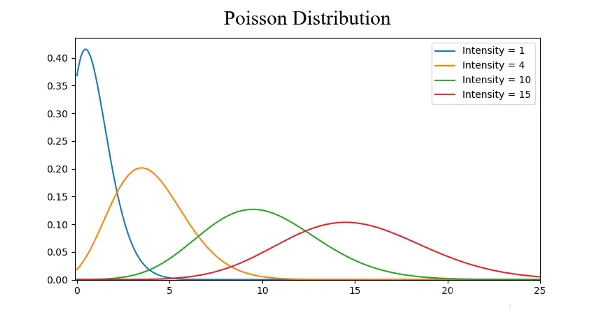
\includegraphics[width=0.55\textwidth]{figs/2022-04-27-09-17-50.png}
      \end{center}
   \[ P(X=k)=\frac{\lambda^{k}}{k !} e^{-\lambda} ; \qquad P (n) =  \frac{ \overline{n} ^{n} e^{-\overline{n}}}{n!} \]
   相干态: $ \rs{\alpha} =  D(\alpha)  \rs{0} $, 
   峰值位置: $ \overline{n} = \left| \alpha\right|^2 $, 展宽(量子涨落): $ \Delta n = \left| \alpha\right| $ 
\end{frame}

\begin{frame}
 \frametitle{场算符的量子涨落}
 \例[10.试证明所有的相干态都是最小不确定度乘积态]{
   \[ \Delta X_1 \Delta X_2 =\dfrac{1}{4} \] 
  }
 \证~湮灭算符不厄密, 总可以写成两厄密算符的如下形式
 \[ a = X_1 + i X_2, \, a ^\dagger = X_1 - i X_2, \qquad \text{with}\qquad  [X_1, X_2]= \frac{i}{2} \]
 对应场的正交分量算符: 
 \[ \hat{X}_{1} =\frac{1}{2}\left(a + a^{\dagger}\right)\]
 \[ \hat{X}_{2} = \frac{1}{2 i}\left(a - a^{\dagger}\right)\]
\end{frame}


\begin{frame}
 \frametitle{}
      先证明对易关系: 
    \[ \begin{aligned}
        \hat{X}_{1} \hat{X}_{2} & =\mathrm{i}\left(\hat{a}^{\dagger}+\hat{a}\right)\left(\hat{a}^{\dagger}-\hat{a}\right) / 4\\ 
        &=\mathrm{i}\left(\hat{a}^{\dagger} \hat{a}^{\dagger}+\hat{a} \hat{a}^{\dagger}-\hat{a}^{\dagger} \hat{a}-\hat{a} \hat{a}\right) / 4 \\ 
        \hat{X}_{2} \hat{X}_{1} & = \mathrm{i}\left(\hat{a}^{\dagger}-\hat{a}\right)\left(\hat{a}^{\dagger}+\hat{a}\right) / 4 \\ 
        & =\mathrm{i}\left(\hat{a}^{\dagger} \hat{a}^{\dagger}-\hat{a} \hat{a}^{\dagger}+\hat{a}^{\dagger} \hat{a}-\hat{a} \hat{a}\right) / 4 \\ 
        \left[\hat{X}_{1}, \hat{X}_{2}\right] & =\hat{X}_{1} \hat{X}_{2}-\hat{X}_{2} \hat{X}_{1} \\ 
        &= \mathrm{i}\left(\hat{a} \hat{a}^{\dagger}-\hat{a}^{\dagger} \hat{a}\right) / 2 \\ 
        & =\mathrm{i}\left[\hat{a}, \hat{a}^{\dagger}\right] / 2  \\ &=  \frac{i}{2} \\ 
        \Delta X_1 \Delta X_2 & \geq  \left| \left[\hat{X}_{1}, \hat{X}_{2}\right]  \right| /2  \\ 
        &= \frac{1}{4}
    \end{aligned}\]

\end{frame}

\begin{frame} 
 \frametitle{}
      电场的行波展开
      \[ \begin{aligned}
          E(\mathbf{r},t)  &= i  \sqrt{\frac{\hbar \omega}{2 \epsilon_0 V}} [a e^{i(\mathbf{k}\cdot \mathbf{r} -\omega t) }- 
          a^{\dagger} e^{-i(\mathbf{k}\cdot \mathbf{r}-\omega t)}]\\
          &=i  \sqrt{\frac{\hbar \omega}{2 \epsilon_0 V}} [X_1 \sin(\mathbf{k}\cdot \mathbf{r}-\omega t) + X_2 \cos(\mathbf{k}\cdot \mathbf{r}-\omega t)] 
      \end{aligned}\] 
      电场的驻波展开
      \[ \begin{aligned}
        E(\mathbf{r},t)  &= \frac{1}{2} E_0 [ a e^{ -\omega t}+ a^{\dagger} e^{ \omega t}] \\ 
        &= E_0 [X_1 \cos(\omega t)+ X_2 \sin(\omega t)]
      \end{aligned}\]
    式中
    \[ X_1 = \sqrt{\frac{\omega}{2\hbar}}q, \qquad X_2 = \sqrt{\frac{1}{2\hbar\omega}}p\]
\end{frame}
\begin{frame} 
    对相干态求均值
    \[
    \begin{aligned}
        \overline{ X_1}  &= \lcr{\alpha}{\frac{1}{2}\left(a+a^{\dagger}\right)}{\alpha} = \frac{1}{2}(\alpha+\alpha^*) \\
        \overline{X_2}  &= \lcr{\alpha}{\frac{1}{2i}\left(a-a^{\dagger}\right)}{\alpha} = \frac{1}{2i}(\alpha-\alpha^*) \\
    \end{aligned}\]
    对相干态求方的均值
    \[
    \begin{aligned}
      \overline{X^2 _1} &= \lcr{\alpha}{\frac{1}{4}\left(a+a^{\dagger}\right)^2} {\alpha}  \\ 
      &= \frac{1}{4}\lcr{\alpha}{\left(aa+a^{\dagger}a^{\dagger}+ aa^{\dagger} + a^{\dagger}a\right)} {\alpha}  \\
      &= \frac{1}{4}\lcr{\alpha}{\left(aa+a^{\dagger}a^{\dagger}+ 2a^{\dagger}a + 1 \right)} {\alpha} \\
      &= \frac{1}{4}(\alpha + \alpha^*)^2+ \frac{1}{4}
    \end{aligned}   
    \]
\end{frame}

\begin{frame}
      \frametitle{}
      \[
        \begin{aligned}
          \overline{X^2 _2} &= \lcr{\alpha}{-\frac{1}{4}\left(a-a^{\dagger}\right)^2} {\alpha}  \\ 
          &= -\frac{1}{4}\lcr{\alpha}{\left(aa+a^{\dagger}a^{\dagger}- aa^{\dagger} - a^{\dagger}a\right)} {\alpha}  \\
          &= -\frac{1}{4}\lcr{\alpha}{\left(aa+a^{\dagger}a^{\dagger}- 2a^{\dagger}a - 1 \right)} {\alpha} \\
          &= -\frac{1}{4}(\alpha - \alpha^*)^2 + \frac{1}{4}
        \end{aligned}   
        \]  
        求场的量子涨落:
        \[ \Delta X_1 = \sqrt{\overline{X^2 _1}- \overline{X_1}^2} = \frac{1}{2}\]
        \[ \Delta X_2 = \sqrt{\overline{X^2 _2}- \overline{X_2}^2} = \frac{1}{2}\]
        \[ \Delta X_1 \Delta X_2=\frac{1}{4}\]
    证毕!
\end{frame}

\begin{frame} 
\frametitle{相干态的相位分布}
对于相干态$\rs{\alpha}$, 取
\[ \alpha = \left|\alpha\right| e^{i\theta}\]
相位分布:
    \[\begin{aligned}
    P(\varphi) &=\frac{1}{2\pi} \left| \lr{\varphi}{\alpha} \right|^2 \\ 
    &= \frac{1}{2\pi} e^{-\left|\alpha\right|^2} \left|  \sum_{n=0} ^{+\infty}  e^{i[n(\varphi-\theta)]}\frac{|\alpha|^n}{\sqrt{n!}} \right|^2
    \end{aligned} \] 
当 $|\alpha|^2$很大时, 泊松分布可近似为高斯分布
\[ e^{-\left|\alpha\right|^2 /2}\frac{|\alpha|^{2n}}{n!} e^{-\left|\alpha\right|^2} \approx \frac{1}{\sqrt{2\pi \left|\alpha\right|^2}} \exp[-\frac{(n-\left|\alpha\right|^2)^2}{2\left|\alpha\right|^2}]\]   
\end{frame}

\begin{frame}
\frametitle{}
\begin{columns}
    \begin{column}[t]{0.6\linewidth}
        ~\\
    相位近似为峰位在$\varphi = \theta$处的高斯分布:
        \[ P(\varphi) \approx \sqrt{\frac{2 \left|\alpha\right|^2}{\pi}} \exp[-2\left|\alpha\right|^2(\varphi - \theta)^2]\]
   很明显,随着 $\left|\alpha\right|^2$的增大, 相位分布集中到$\varphi = \theta$附近。即相位变得越来越确定, 相干态趋相于经典态。
    \end{column}
    \begin{column}[t]{0.4\linewidth} 
          \begin{center}
               
\includegraphics[width=1.0\textwidth]{figs/33.png} 
          \end{center} 
    \end{column} 
\end{columns} 
\end{frame}

\begin{frame}
      \frametitle{相干态的相图}
    与真空态不同, 相干态的场矢量大小为$\left|\alpha\right|$, 是平移量的模! 
   \begin{center}
        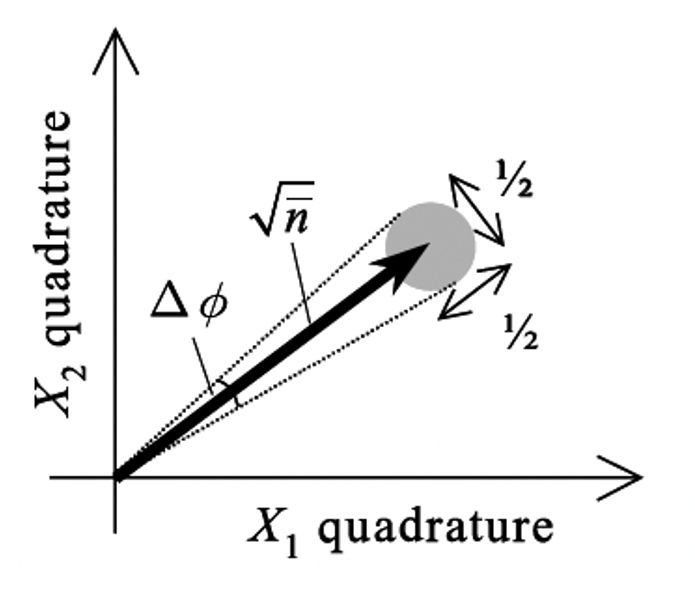
\includegraphics[width=0.35\textwidth]{figs/13.png}
   \end{center}
   相干态是真空态的幺正平移,因此涨落性质不变!\\ 
   但随着场强增大,其相位的不确定度从真空态的无限大变得越来越小,\\ 当场强足够大时, 相位的不确定度趋零,对应于有确定相位的经典电磁场.
\end{frame}

\begin{frame}
    \frametitle{相干态的产生}
  理论上,得要构造一个系统, 具有如下平移算符. 
  \[ D(\alpha)=\exp \left(\alpha a^{\dagger}-\alpha^{*} a\right) \]
  ~\\ {\vspace*{2.3em}} 
  实验上:\\
  (1)电流源辐射: 激发(平移)真空态产生相干辐射场.
\end{frame}

\begin{frame}
    ~\\
   (2)原子受激辐射: 大量同一种原子受激辐射, 产生与激源光子物理特性完全相同的光(激光).  
     \begin{center}
      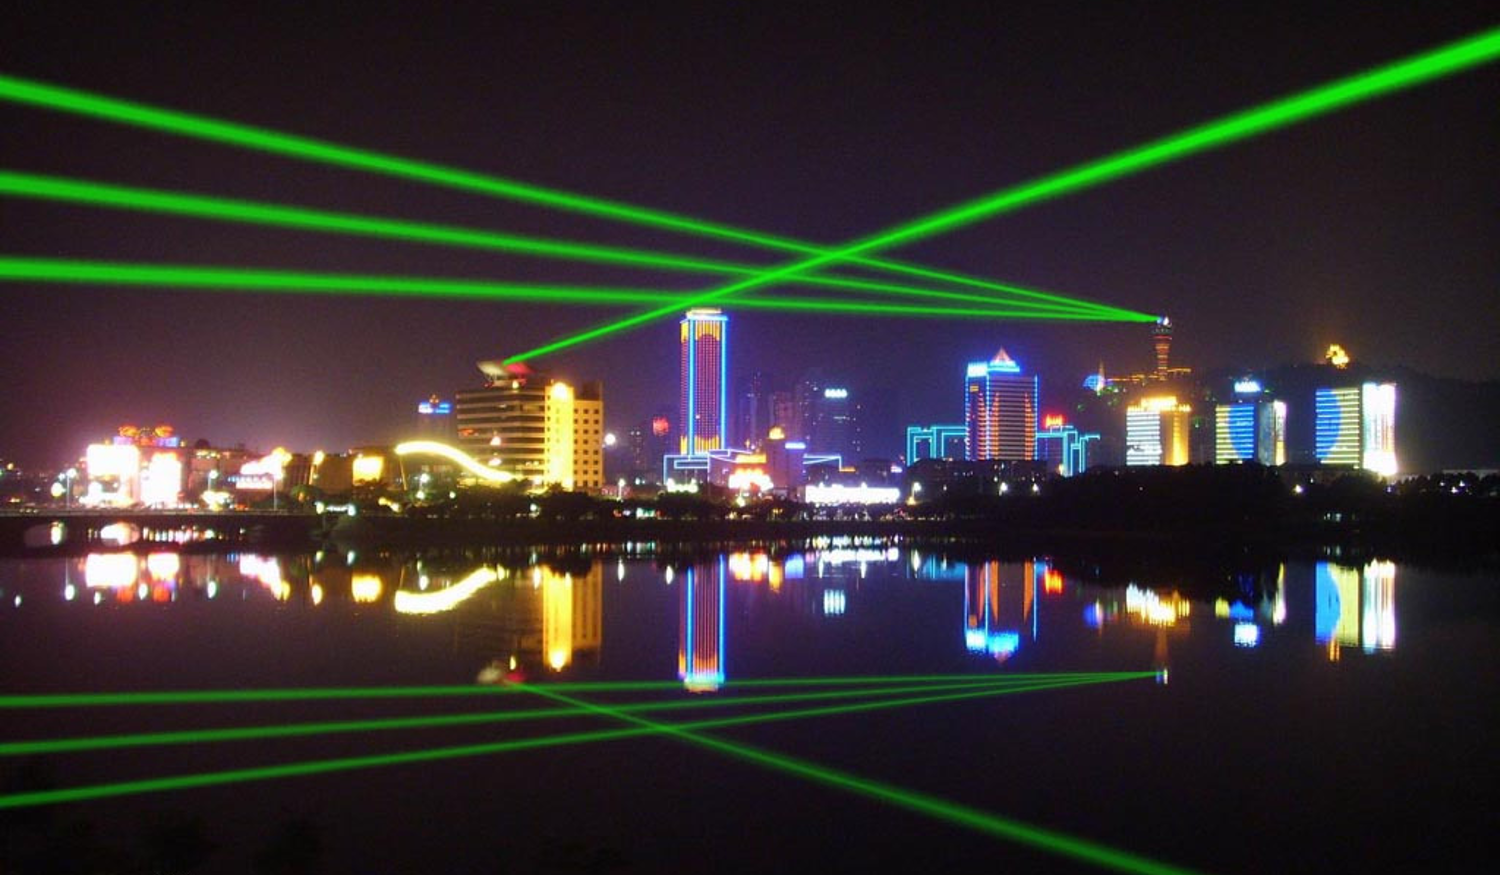
\includegraphics[width=0.35\textwidth]{figs/8.png}
    \end{center}   
 原子自发辐射发的光子,不具有相位、偏振态、传播方向上的一致性,是非相干光. 当有信号光子入射时, 处于高能级的原子可辐射一个与信号光子频率、相位、偏振态以及传播方向都相同的光子. 如果大量原子被激励(平移)到高能级,则可产生大量频率、相位、偏振态以及传播方向相同的相干光.  
\end{frame}

\begin{frame}
    \frametitle{相干态随时间的演化规律}
        \例[11. 已知$t=0$时刻的相干态为$\rs{\alpha (0)}$, 试求t时刻的相干态$\rs{\alpha (t)}$  ]{}
        \解 ~ 设光场哈密顿不显含时间, 其时间演化算符为
    \[ \begin{aligned}
     \hat{U}(t, 0)  &= e^{-i \hat{H}t / \hbar}\\ 
     &= e^{-i \hbar \omega ( a^\dagger a+\frac{1}{2} ) t / \hbar} \\ 
     &= e^{-i \omega t (a^\dagger a +\frac{1}{2} )}  \\ 
    \end{aligned}\]
    数态表象:
    \[ \begin{aligned}
        \rs{\alpha (t)} &= \hat{U}(t, 0) \rs{\alpha (0)} \\ 
        &= e^{-i \omega t ( a^\dagger a +\frac{1}{2} )} \rs{\alpha (0)} \\ 
        &= e^{-i \omega t ( a^\dagger a +\frac{1}{2} )} e^{-\frac{1}{2}\left|\alpha(0)\right|^2}  \sum_{n=0} ^{+\infty}  \frac{\alpha(0)^n}{\sqrt{n!}} \rs{n}  \\  
       \end{aligned}\]
\end{frame}

\begin{frame}
    \frametitle{}
    \[ \begin{aligned}
        \rs{\alpha (t)} &= e^{-i\frac{1}{2} \omega t}  e^{-\frac{1}{2}\left|\alpha(0)\right|^2} \sum_{n=0} ^{+\infty}  \frac{\alpha(0)^n}{\sqrt{n!}} e^{-i \omega t  a^\dagger a}  \rs{n}  \\
        &= e^{-i\frac{1}{2} \omega t}  e^{-\frac{1}{2}\left|\alpha(0)\right|^2}\sum_{n=0} ^{+\infty}  \frac{\alpha(0)^n}{\sqrt{n!}} e^{-i n \omega t }  \rs{n}  \\ 
        &= e^{-i\frac{1}{2} \omega t}  e^{-\frac{1}{2}\left|\alpha(0)\right|^2} \sum_{n=0} ^{+\infty}  \frac{(\alpha(0) e^{-i \omega t })^n}{\sqrt{n!}} \rs{n}  \\ 
        &= e^{-i\frac{1}{2} \omega t} e^{\left|e^{-i \omega t }\right|^2}   e^{-\frac{1}{2}\left|\alpha(0)e^{-i \omega t }\right|^2} \sum_{n=0} ^{+\infty}  \frac{(\alpha(0) e^{-i \omega t })^n}{\sqrt{n!}} \rs{n}  \\ 
        &= e^{-i\frac{1}{2} \omega t}  e^{\left|e^{-i \omega t }\right|^2}  \rs{\alpha(0) e^{-i \omega t} } \\ 
        &= \rs{\alpha(0) e^{-i \omega t}} \\ 
       \end{aligned}\]
\end{frame}

\begin{frame}
      \frametitle{}
      \[ \rs{\alpha (t)}= \rs{\alpha(0) e^{-i \omega t}}  \]
       说明: 随着时间的推移, 相干态的本征值只是获得一个相位 $e^{-i \omega t}$, 相干态本身变成了湮灭算符的属于本征值$ \alpha(0) e^{-i \omega t} $的本征态. \\ {\vspace*{0.6em}} 
       即, 随着时间的推移, 相干态只是获得一个相位振荡, 它还是湮灭算符的本征态, 所以相干特性不随时间发生变化. 这正是实验上发现稳定相干条纹的前提.
\end{frame}

\begin{frame}
 \frametitle{}
    \begin{center}
    \animategraphics[height=2in,loop]{30}{gif/coh-}{1}{100} 
    \end{center}
    相干态在相图中表现为:
 \begin{enumerate}
     \item 场矢大小保持不变
     \item 相位随时间发生周期性振荡(频率$\omega$)
 \end{enumerate}
\end{frame}

\begin{frame} 
\frametitle{}
    \begin{center}
    \animategraphics[height=2in,loop]{30}{gif/test-}{1}{80} 
    \end{center} 
相干态在位置表象表现为: 
\begin{enumerate}
  \item 波包的形状保持不变
  \item 在中心位置附近做周期性振荡(频率$\omega$)
\end{enumerate}  
\end{frame}

\section{5. 相干态表象}

\begin{frame}
    \frametitle{相干态不正交}
        \例[12.试证明相干态不具正交性]{}
        \证 ~ 相干态
        \[\rs{\alpha}=e^{-\frac{1}{2}\left|\alpha\right|^2}  \sum_{n=0} ^{+\infty}  \frac{(\alpha\hat{a}^\dagger)^n}{n!}\rs{0} \] 
    代入内积公式
    \[ \begin{aligned}
     \lr{\alpha}{\beta} &= \lr{0\left|\sum_{n=0} ^{+\infty}\frac{(\alpha\hat{a}^\dagger)^n}{n!}}{\sum_{n=0} ^{+\infty}\frac{(\beta\hat{a}^\dagger)^n}{n!}\right|0} e^{-\frac{1}{2}(\left|\alpha\right|^2 +\left|\beta\right|^2)}\\ 
     &= e^{-\frac{1}{2}(\left|\alpha\right|^2 +\left|\beta\right|^2)} \sum_{n=0} ^{+\infty}\frac{(\alpha^*)^n (\beta)^n}{n!} \\ 
     &= e^{\alpha^* \beta -\frac{1}{2}(\left|\alpha\right|^2 +\left|\beta\right|^2)} \\ 
     \left|\lr{\alpha}{\beta} \right|^2 &= e^{-  \left| \alpha - \beta\right|^2} \not = 0 
    \end{aligned}\]
\end{frame}

\begin{frame}
    Analysing the two-slit experiment:
      \begin{center}
           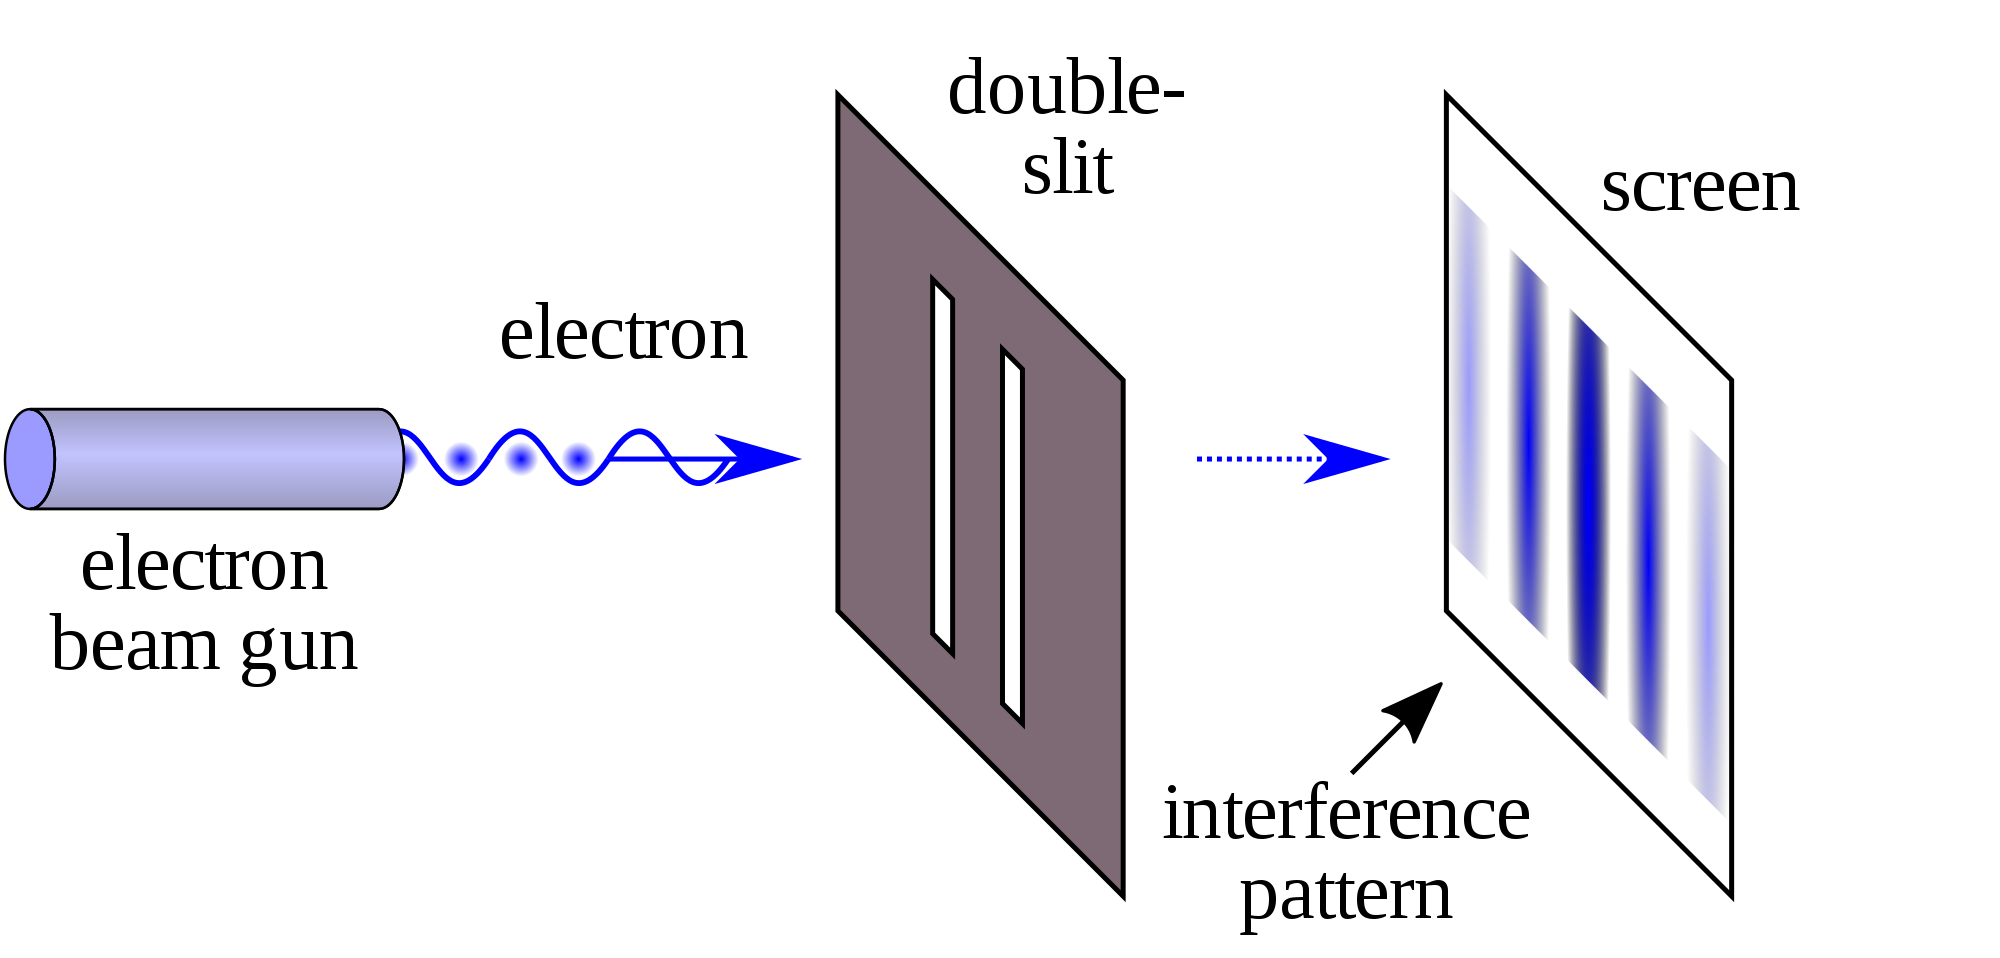
\includegraphics[width=0.6\textwidth]{figs/Etwoslitexp.png}
      \end{center}
    \begin{itemize}
        \Item Using wavefunction $\rs{\psi_1}$ to describe the state of the electron running across slit-1 and $\rs{\psi_2}$ for slit-2. when the both slits opened, the electron locates at the superposition state
            \[ \rs{\Psi}=c_1 \rs{\psi_1}+ c_2\rs{\psi_2} \]
    \end{itemize}
\end{frame}

\begin{frame}
    \tikzstyle{na} = [baseline=-.5ex]
    \begin{itemize}
        \Item based on statistical interpretation, the possiblity density of electron reaches certain point of screen should be
        \begin{equation*}
        \begin{split}
            \omega &=|\rs{\Psi}|^2 \\
            &= (\ls{\psi_1}c_1 + \ls{\psi_2}c_2 ) (c_1 \lr{\psi_1}+ c_2\lr{\psi_2}) \\
            & = |c_1|^2 |\rs{\psi_1}|^2 + |c_2|^2 |\rs{\psi_2}|^2  
            + \Myitem{t1}{red}{c_1 c_2 ^* \lr{\psi_2}{\psi_1} + c_1 ^* c_2 \lr{\psi_1}{\psi_2} } \\
        \end{split} 
        \end{equation*}
    \end{itemize}
    \begin{itemize}
        \Item 存在相干项(后两项),形成干涉条纹
        \Item 相干项不为零的条件: 
        \begin{enumerate}
            \item 叠加态: 即同时过两个缝, 否则有$\psi_1$ 或$\psi_2$为零,相干项为零
            \item 不正交性: $\rs{\psi_1}$与 $\rs{\psi_2}$不正交, 否则相干项为零
        \end{enumerate}
        \Item $\left|\lr{\alpha}{\beta} \right|^2 = e^{-  \left| \alpha - \beta\right|^2}$ 表明, 当$\alpha - \beta \to \infty $, 
        趋于正交, 相干项趋零.
    \end{itemize}
\end{frame}

\begin{frame}
 \frametitle{}
   \begin{center}
        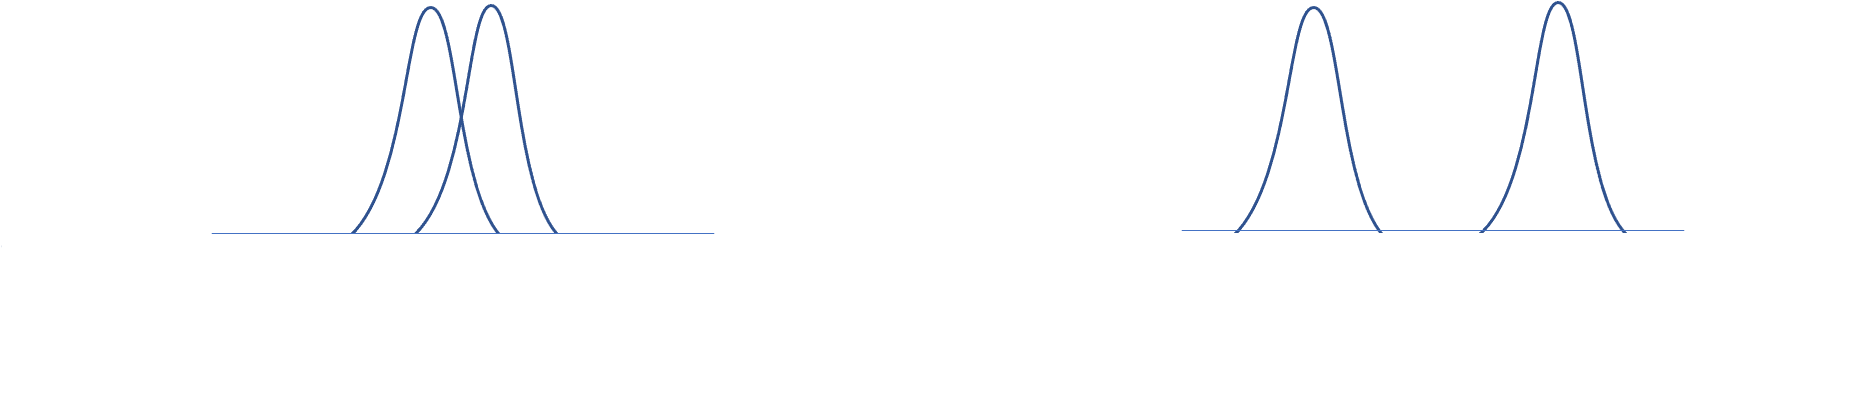
\includegraphics[width=1.0\textwidth]{figs/11.png}
   \end{center}
 当$\alpha - \beta \to \infty $, 两位移量差别大, 两波函数虽不正交但振荡过程中相互重叠部分趋零, 因此内积趋零, 干涉项趋零, 干涉条纹变弱趋无。
 
\end{frame}

\begin{frame}
 \frametitle{相干态的超完备性}
 \例[13.试证明相干态具有如下完备性关系]{
    \[ \frac{1}{\pi} \int \rl{\alpha}{\alpha}d ^2 \alpha =1 \] }
 \证 ~ 把相干态的数态展开式
    \[\rs{\alpha} = e^{-\frac{1}{2}\left|\alpha\right|^2}  \sum_{n=0} ^{+\infty}  \frac{\alpha^n}{\sqrt{n!}} \rs{n} \]
 代入上式左边:
 \[
    \begin{aligned}
        \frac{1}{\pi} \int \rl{\alpha}{\alpha}d ^2 \alpha &=  \frac{1}{\pi} \int \sum_{n,m=0} ^{+\infty} e^{-\left|\alpha\right|^2}  
        \frac{\alpha^n(\alpha^*)^m}{\sqrt{n!m!}}  \rs{n}\ls{m }d ^2 \alpha \\
        &= \sum_{n,m=0} ^{+\infty}  \frac{\rs{n}\ls{m }}{\pi \sqrt{ n!m!}}  \int  e^{-\left|\alpha\right|^2}  \alpha^n(\alpha^*)^m  d ^2 \alpha
    \end{aligned}    
 \]    
\end{frame}

\begin{frame}
 \frametitle{}
  转换到极坐标系进行计算
  \[ 
    \begin{aligned}
        \frac{1}{\pi} \int \rl{\alpha}{\alpha}d ^2 \alpha 
        &= \sum_{n,m=0} ^{+\infty}  \frac{\rs{n}\ls{m }}{\pi \sqrt{ n!m!}}  \int  e^{-\left|\alpha\right|^2}  \alpha^n(\alpha^*)^m  d ^2 \alpha \\ 
        &= \sum_{n,m=0} ^{+\infty}  \frac{\rs{n}\ls{m }}{\pi \sqrt{ n!m!}} 
        \int _0 ^ {+\infty}  e^{-r^2}  r^{n+m}  r dr   \int _0 ^ {2 \pi} e^{i(n-m)\theta} d\theta  \\ 
        &= \sum_{n,m=0} ^{+\infty}  \frac{\rs{n}\ls{m }}{\pi \sqrt{ n!m!}} 
        \int _0 ^ {+\infty}  e^{-r^2}  r^{n+m}  r dr   2 \pi \delta(n-m)  \\ 
        &= \sum_{n=0} ^{+\infty}  \frac{\rs{n}\ls{n }}{\sqrt{ n!n!}} 
        \int _0 ^ {+\infty}  e^{-r^2}  r^{n+n}  2r dr  \\ 
        &= \sum_{n=0} ^{+\infty}  \frac{\rs{n}\ls{n }}{n!} 
        \int _0 ^ {+\infty}  e^{-(r^2)}  (r^2)^{n}   d(r^2)  
    \end{aligned}    
 \]        
\end{frame}

\begin{frame}
 \frametitle{}
 \[ 
    \begin{aligned}
        \frac{1}{\pi} \int \rl{\alpha}{\alpha}d ^2 \alpha    
        &= \sum_{n=0} ^{+\infty}  \frac{\rs{n}\ls{n }}{n!} 
        \int _0 ^ {+\infty}  e^{-t}  t^n   dt  \\ 
        &= \sum_{n=0} ^{+\infty}  \frac{\rs{n}\ls{n }}{n!} 
        \Gamma(n+1)  \\ 
        &= \sum_{n=0} ^{+\infty}  \frac{\rs{n}\ls{n }}{n!} 
        n!  \\ 
        &= \sum_{n=0} ^{+\infty}  \rs{n}\ls{n } \\
        &= 1
    \end{aligned}    
 \] 
 证毕!
\[  \boxed{ \frac{1}{\pi} \int \rl{\alpha}{\alpha}d ^2 \alpha =1} \]
\end{frame}

\begin{frame} 
\frametitle{}
     * 相干态表象的过完备性: $\{\rs{\alpha}\}$的一个子集就可以构成一组完备基, 因此一个态函数在相干态表象中的展开系数是不唯一的.也称超完备性. \\ {\vspace*{0.3em}}
     \证~(1)线性不独立性
     \[ \begin{aligned}
         \int \alpha ^m \rs{\alpha} d^2 \alpha &= \sum_n \frac{\rs{n}}{\sqrt{n!}} \int_0 ^\infty \left|\alpha\right|^{n+m+1} e ^ {- \left|\alpha\right|^2 /2} \int_0 ^{2\pi} e ^{i(n+m)\varphi}  d \varphi =0\\
     \end{aligned}\] 
     (2) 相干态可以相互展开
     \[ \begin{aligned}
        \rs{ \beta } & = \frac{1}{\pi} \int \rs{\alpha} \left\langle \alpha | \beta \right\rangle  d ^2 \alpha \\ 
        &= \frac{1}{\pi} \int \rs{\alpha} e^{-  \left| \alpha - \beta\right|^2}  d ^2 \alpha
    \end{aligned}\] 
\end{frame}

\begin{frame} 
\frametitle{}
     (3) 对于$\{\rs{\alpha}\}$,设$\alpha = r e ^{i \varphi}$, 则$r$取一个固定值的子集就是一组完备基
      \[ \begin{aligned}
          \int _0 ^{2\pi} \rs{\alpha} e ^{-i m \varphi} d \varphi &= e^{- r^2 /2 \sum_n \frac{\rs{n} r^n}{\sqrt{n!}} } \int _0 ^{2\pi} e ^{i (n-m) \varphi} d \varphi \\
          &= 2\pi r^m e^{- r^2 /2}  \frac{\rs{m}}{\sqrt{m!}} \\
        \to \rs{m} &= \frac{r^{-m}}{2\pi}e^{ r^2 /2}  \int _0 ^{2\pi} \rs{\alpha} e ^{-i m \varphi} d \varphi 
      \end{aligned}\] 
      数态可以在这个子集上展开, 因此是完备的. 
\end{frame}

\begin{frame} 
\frametitle{}
      (4) 算符在相干态表象中的矩阵表示是不唯一的.
    \[\begin{aligned}
         F_{\alpha' \alpha} &= \left\langle \alpha' | F |\alpha \right\rangle \\ 
         &= \sum_m \sum_n  \left\langle \alpha' |m \right\rangle F_{mn} \left\langle n |\alpha \right\rangle \\
         &= F(\alpha^*, \alpha')e^{-(\left|\alpha\right|^2+ \left|\alpha'\right|^2)/2}  
    \end{aligned} \]
      式中 \[F(\alpha^*, \alpha')= \sum_m \sum_n F_{mn} \frac{(\alpha^*)^m (\alpha)^n}{\sqrt{m! n!}}\]
     称矩阵元的生成函数.
\end{frame}

\begin{frame} 
\frametitle{}
    (5)对角元已具有完全性 \\ {\vspace*{0.6em}}
      上式取$\alpha'=\alpha$, 得相干态表象矩阵的对角元。
      \[ \left\langle \alpha|F|\alpha \right\rangle\]
      通过这些对角元即可生成数态表象中的整个矩阵
      \[ \left\langle \alpha|F|\alpha \right\rangle e^{\alpha^* \alpha} = \sum_m \sum_n  \frac{(\alpha^*)^m (\alpha)^n}{\sqrt{m! n!}} \left\langle m|F|n \right\rangle\]
\end{frame}

\begin{frame} 
 \frametitle{}
        \begin{center}
             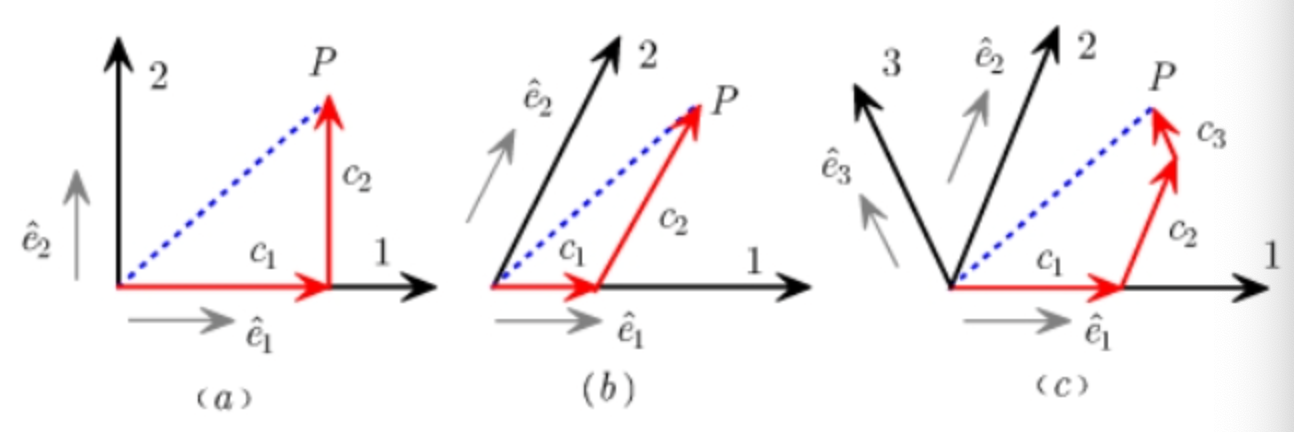
\includegraphics[width=1.0\textwidth]{figs/2022-05-11-11-10-06.png}
        \end{center}
    \begin{enumerate}
        \item 正交完备空间~表述唯一
        \item 非正交完备空间~表述唯一
        \item 非正交超完备空间~表述不唯一
    \end{enumerate}
\end{frame}

%%%%%%%%%%%%%%%%%%%%%%%%%%%%%%%%%%%%%%%%%%%%%%%%%%%%%%%%%%%%%%%%%%%
\begin{frame}
    \frametitle{课外作业}
    \begin{enumerate}
        \item 试证明相干态是最小不确定度乘积态
        \item 试求相干态在位置表象中的波函数
        \item 试求位置表像里,相干态随时间的振荡表达式
        \item 证明
        \[D^\dagger (\alpha) a^\dagger D (\alpha) = a^\dagger + \alpha^* \]
        \[ \rs{\alpha }\ls{\alpha } a= \left( \alpha + \frac{\partial }{\partial \alpha^*} \rs{\alpha }\ls{\alpha } \right)\]
    \end{enumerate}
\end{frame}
%%%%%%%%%%%%%%%%%%%%%%%%%%%%%%%%%%%%%%%%%%%%%%%%%%%%%%%%%%%%%%%%%%